\chapter{Intonation: Theory and typology}
%\chapter{Intonation and the phonetic implementation of tone}
% Intonation in a level-tone language: Phonetic realization and tonal Processes
%\chapter{From surface phonological tone to phonetic realization}
\label{chap:IntonationTheoryAndTypology}

\is{intonation|(}


\epigraph{{\dots}~a~theory of tone must provide some means for describing intonational processes independently of tonal patterns, as well as a~procedure for integrating the two structures.}{\citep[547]{clements1979}}

\epigraph{If, as seems to be the case, the complexity of intonation is typical of human complexity, then there is still a~long way to go before ({\dots}) intonation yields all of its secrets.}{\citep[256]{vaissiere2004}}


%\section{Introduction}
%\label{sec:introductionsurfacetoreal} %%% Never mentioned elsewhere, it's OK to comment out

%In retrospect, I should clarify that the real reason for avoiding the term \textit{intonation} in the chapter title was my concern that the book manuscript as a~whole might be rejected for not adhering to ``the now widely accepted “autosegmental-metrical” theory of intonation", as it is called in an article on ``Prosodic description: an introduction for fieldworkers" \citep{himmelmann_prosodic_2008} published in \textit{Language Documentation and Conservation}. From experience, I knew that engaging critically with the mainstream generative approach to intonation could, in itself, be a red flag, potentially obstructing publication. In this second edition, the chapter's title is finally brought into alignment with its actual contents.
% providing an account of Na intonation without forcing it into an autosegmental-metrical model 
% stating my doubts about the mainstream model, and my observation that this model did more harm than good as a~tool for language description

The field of intonation studies remains characterized by a diversity of seemingly irreconcilable approaches~-- an inexhaustible source of misunderstandings. The detailed discussion of various frameworks in \citet{prosodic_2022} suggests that little progress has been made in resolving these differences since \citet{dicristo1998} examined them nearly three decades ago. 
%\footnote{This section contains passages adapted from \citet{michaud_et_al_intonation_2021}.}

\begin{quotation}
Researchers, we have noticed, often use shared terminology in subtly different ways. These differences, frequently stemming from underlying differences in the goals researchers have set for themselves and
    their models, are also often either unacknowledged or unexplored by researchers, whose
    subsequent disagreements are animated precisely by these unspoken divergences. \citep[1]{barnes2022}
\end{quotation}

In view of this persistent lack of consensus, 
%before going into an analysis of salient characteristics of Na intonation (in the next chapter), 
it is necessary to address some conceptual issues. 
Are intonational phenomena best analyzed using the same theoretical constructs as lexical tone, or do they require an entirely separate framework? Should intonation be conceived primarily in terms of phonological categories, or does it have ties to other areas of language structure~-- such as morphology, syntax, and pragmatics~-- that call for a~more pluridisciplinary approach? Divergent answers to these questions have led to competing models that, rather than converging towards a~unified account, have continued to evolve along largely parallel trajectories. 

Against this backdrop, careful reflection on the choice of framework and the definition of key terms~-- beginning with the notion of intonation itself~-- appears indispensable. This chapter engages with the theoretical landscape of intonation studies, establishing theoretical and typological foundations through an open discussion of the key issues at stake. The next chapter (Chapter~\ref{chap:IntonationDescriptionAndAnalysis}) turns to the specifics of Yongning Na, presenting the detailed empirical work delving into its intonation system as well as issues of phonetic implementation.
%it appears indispensable to take the time to reflect carefully on the choice of framework and the definition of key terms, beginning with the notion of intonation itself. 

This chapter does not seek to provide a comprehensive survey of existing models~-- an endeavour that would go beyond the scope of this work~-- but instead aims to clarify the theoretical choices adopted in this study. \sectref{sec:PhonStarDefOfIntonation} examines the limitations of phonetic-phonological definitions of intonation, which tend to be too narrow in scope. In \sectref{sec:IssuesWithATonalDescriptionOfIntonation}, I critically assess approaches that have influenced recent research, particularly the autosegmental-metrical framework. A~central argument of this chapter is that this widely used model is not ideally suited for tonal languages. Section \sectref{sec:intonationaltypology} explores the typological distinction between tonal and non-tonal intonation, emphasizing its crucial importance to intonational typology. 
%I then addresses issues with tonal descriptions of intonation, emphasizing the need to distinguish between \textit{tonal intonation} and \textit{non-tonal intonation}. These reflections lead to a~broader perspective on intonational typology, considering the topic of tonal vs.\ non-tonal intonation as subject-matter for intonational typology, explored in \sectref{sec:intonationaltypology}.

Building on this critical discussion, \sectref{sec:ChoiceOfFramework} proposes a~constructive approach, outlining what I consider a~sound foundation for advancing the study of intonation. 
%As many readers will have anticipated, our starting point is a functional characterization, rather than a phonetic-phonological one. 



\section{Issues with a phonetic-phonological definition of intonation}
%\section{A framework for studying intonation}
\label{sec:PhonStarDefOfIntonation}

In his book simply titled  \textit{Intonation}, Alan Cruttenden begins by defining a `supra\-segmental' domain (also referred to as the `prosodic' domain), which he contrasts~-- following a~long-standing tradition~-- with the segmental domain, that of phonemes. For instance, the adjective \textit{nice} consists of three phonemes: a nasal consonant /n/, a diphthong /aɪ/, and a fricative /s/. This constitutes its segmental composition: /naɪs/. 

\begin{quotation}
    But there are clearly other features involved in the way a word is said which are not indicated in a segmental transcription. The word \textit{nice} might be said softly or loudly; it might be said with a pitch pattern which starts high and ends low, or with one which begins low and ends high; it might be said with a voice quality which is especially creaky or especially breathy. Such features generally extend over stretches of utterances longer than just one sound and are hence often referred to as suprasegmentals ({\dots}). Alternatively, the shorter term \textsc{prosodic} is sometimes used and I shall generally prefer this term in this book. \citep[1]{cruttenden1986}
\end{quotation}

So far, intonation has not been explicitly mentioned. It makes a discreet entrance in the following sentence, parenthetically.

\begin{quotation}
    Prosodic features may extend over varying domains: sometimes over relatively short stretches of utterances, like one syllable or one morpheme or one word ({\dots}); sometimes over relatively longer stretches of utterances, like one phrase, or one clause, or one sentence (intonation is generally relatable to such longer domains). \citep[1]{cruttenden1986}
\end{quotation}

These two extended quotations highlight a paradoxical observation: Alan Cruttenden does not provide a~definition of intonation, as if the meaning of the term were self-evident. He contrasts the \textit{segmental} dimension of an utterance (its consonants and vowels) with its \textit{suprasegmental} features, suggesting that the latter have a structure of their own. The phrase ‘prosodic features’ implies that prosody is organized into discrete units~-- features, a fundamental concept in phonology \citep[182]{martinet1955}. Within the domain of prosodic features, one is left to infer that only some are intonational in nature. Readers of Cruttenden's textbook are left to determine for themselves, as they progress through the text, what is actually meant by `intonation'. Are we to understand that intonation is an abstract linguistic structure pertaining to non-segmental units? 

In an encyclopaedia article carrying the same title, ‘Intonation’, Francis Nolan provides a more explicit characterization. 

\begin{quotation}
    The term intonation refers to a means for conveying information in speech which is independent of the words and their sounds. Central to intonation is the modulation of pitch, and intonation is often thought of as the use of pitch over the domain of the utterance. However, the patterning of pitch in speech is so closely bound to patterns of timing and loudness, and sometimes voice quality, that we cannot consider pitch in isolation from these other dimensions. ({\dots}) For those who prefer to reserve ‘intonation’ for pitch effects in speech, the word ‘prosody’ is convenient as a more general term to include patterns of pitch, timing, loudness, and (sometimes) voice quality. \citep[433]{nolan_intonation_2006} 
\end{quotation}

In this passage, the negative characterization of intonation as a domain independent of phonemes is enriched by an important observation concerning the level of the word. Stating that intonation is ``independent of the words and their sounds'' clarifies that intonation operates above the level of the word, and therefore above lexical phenomena such as accent (in a language like English) and tone (in languages such as \ili{Bambara}, \ili{Mandarin} or Yongning Na). However, Francis Nolan does not explicitly describe intonation as an abstract structure; rather, his characterization remains grounded in the idea that intonation is essentially a matter of how spoken communication employs the three acoustic parameters of fundamental frequency (and its perceptual counterpart, pitch), intensity, and duration. 

Confident in the effectiveness of a method that had already proved its worth in the ‘segmental’ domain, many linguists pursued the study of intonation as a problem of phonology. Their aim has been to discern, beneath the seemingly infinite variation of phonetic substance, a structure based on discrete (categorical) oppositions. Beginners seeking introductory reading on intonation are typically directed to works on the \textit{phonology of intonation}, also referred to as \textit{intonational phonology} (discussed further in the next section, \sectref{sec:theabsenceoffullysatisfactorytoolsforintonationaltranscription}).
%\citep{gussenhoven2002,jun2005,ladd2008} 
The phonetician-phonologist tells us ``what intonation consists of, and how we can visualize it and analyze it phonologically" \citep[434]{nolan_intonation_2006}. 

At first glance, this approach aligns with the principles of the scientific method: it is rooted in empirical observation of phonetic phenomena (in particular, the analysis of fundamental frequency curves, which, for English, are regarded as the primary correlate of intonation) and guided by a~commitment to theoretical generalizations. Phonological analysis is seen as the culmination of a process that begins with experimental phonetics and ultimately leads to phonological modelling.

A~careful reader, however, will detect indications that phonetic-phonological approaches to intonation encounter certain limitations~-- limitations that scholars acknowledge without fully drawing out their implications. David Crystal notes that ``intonation is not a single system of contours and levels, but the product of the interaction of features from different prosodic systems~-- tone, pitch-range, loudness, \is{rhythm}rhythmicality and tempo in particular" \citep[11]{crystal_english_1975}. This remark suggests the need to move beyond a~view that reduces intonation to melodic properties alone~-- namely, contours (rises and falls) and levels (on a pitch scale). The reference to ``different prosodic systems'' opens the door to recognizing multiple dimensions of intonation, each of which could, in principle, be approached with its own distinct methods. However, this opening is immediately narrowed to the familiar phonetic dimensions commonly described as ``suprasegmental'' \citep{lehiste1970}, much as they were in Nolan's characterization of intonation quoted above: F\textsubscript{0}, intensity, and duration. While this list is formally open-ended (as signalled by the phrase ‘in particular{\dots}’), in practice it highlights three specific phonetic dimensions~-- ones that naturally lend themselves to phonetic-phonological study.
%\footnote{David Crystal's quote currently appears in the introduction to the article ‘Intonation’ on Wikipedia. It was introduced there by Peter Roach~-- the author of reference works: in particular \citet{roach_english_1983}~--, as part of a vigorous rewrite of this article in February 2013: see \url{https://en.wikipedia.org/w/index.php?title=Intonation_(linguistics)\&oldid=538882783}. Eight years later, around a hundred users had intervened on the article, but despite changes of all kinds, the quotation introduced by Roach still appeared in the article, which suggests that it enjoys consensus.} 

% \footnote{Similarly, the \textit{parallel encoding and
% target approximation} (PENTA) model \citep{xu2005speech} is based on the explicit assumption ``that prosody conveys multiple layers of information simultaneously, through encoding schemes that are in parallel to each other" \citep[377]{penta_2022}, yet in practice it is not always clear to what extent proponents of this model are ready to draw out the full consequences of this approach.}

Once one has come to believe that intonation can be held under one's gaze and brought under phonological scrutiny (to paraphrase Francis Nolan's formulation cited above: ``how we can visualize it and analyze it phonologically"), it is difficult to relinquish the hope of such quasi-immediate access. This expectation is all the more deeply ingrained given that the intonation of English~-- the most widely taught language, and consequently the most extensively studied by linguists~-- can be described more readily than that of many other languages in terms of patterns of fundamental frequency, known as ‘tones’ or ‘tunes’ in the British tradition of intonation studies \citep{oconnoretal1973}. 

Practitioners of language description, however, point out that studying intonation is far from straightforward.

\begin{quotation}
	This phenomenon [=intonation] plays a crucial role in spoken communication, yet its specific properties pose considerable challenges for the linguist, since the methods that have proved their worth in other areas do not appear to be fully suited to the analysis of intonation. \citep[173]{creissels1994}
        
    \medskip 
    %\footnote{
    {\noindent}\textit{Original text:} L'importance de ce phénomène [=l'{intonation}] dans la communication orale est considérable, mais sa spécificité gêne beaucoup le linguiste, car les méthodes d'analyse qui ont fait leurs preuves dans d'autres domaines ne semblent pas convenir vraiment pour l'analyse de l'{intonation}.
\end{quotation}


Is the phonetician-phonologist well-equipped to tackle the complex domain of intonation? The question may seem surprising, given the seemingly evident connection between intonation (which is inherently linked to spoken language) and phonetics-phonology. However, to the extent that, as Pierre Cotte writes, behind the proclaimed ideal of objectivity, ``we do linguistics in a~thoroughly subjective way, and our temperament dictates our approach'' \citep{cotte1993}, it may be worth asking why one chooses to become a phonetician-phonologist. To devote oneself to the study of the sound structure of language is to embrace an area of linguistic inquiry that appears particularly amenable to rigorous analysis, whether in diachronic phonology, synchronic phonology or experimental phonetics. The best generalizations of historical phonetics achieve remarkable levels of precision, even if they allow for important exceptions in detail; it is difficult to match this degree of demonstrable rigour in pragmatics, semantics or even syntax. As for synchronic phonology, it is a favoured domain for those drawn to mathematical models~-- even if the rigour of such models is sometimes more apparent than real \citep{karttunen2006}. Experimental phonetics, the other facet of the \textit{Janus bifrons} that is phonetics-phonology, deploys an impressive experimental apparatus (see, for example, \citealt{vaissiereetal2010,gick_quantal_2020}), which, by positioning the researcher as an external observer, may lessen the necessity of engaging with languages as instruments of communication. It is entirely possible to describe a~phonological opposition without speaking the language in which it occurs~-- an approach widely practised by Peter Ladefoged, for example \citep{ladefogedetal1996}. 

The purpose of these remarks is neither to question the considerable value of such work nor to dispute the fact that a phonetician-phonologist may experience languages in the way many linguists do (in his autobiography, Martinet uses the expression `living out languages': \citealt{martinet1993}). Rather, the point is to highlight a~general tendency: phoneticians-phonologists are not typically among the most generalist of linguists; they are not necessarily the best informed about the full range of linguistic diversity. This makes it paradoxical to entrust phonologists with the task of elucidating how intonation functions, since the study of this domain requires attention to communicative dimensions that are not exclusively (or even primarily) phonetic-phonological. This observation may explain an important part of the considerable discrepancies between different authors' views on intonation.

\section{Issues with tonal models of intonation}
\label{sec:IssuesWithATonalDescriptionOfIntonation}
\label{sec:theabsenceoffullysatisfactorytoolsforintonationaltranscription} %xyz replace this label for references

In addition to what appears in retrospect as a~somewhat too exclusive focus on phonetic and phonological aspects, an additional hurdle in the study of intonation~-- particularly in tonal languages~-- has been the widespread adoption of tonal models for describing intonation. This tendency has shaped the field in ways that warrant careful reconsideration. Given this context, the following arguments need to be made to lay a solid theoretical foundation for the present descriptive work: 

\begin{itemize}
    \item A clear distinction needs to be maintained between \textit{tonal intonation} and \textit{non-tonal intonation}.
    \item The presence or absence of \isi{intonational tones} is a typological parameter that varies across languages.
\end{itemize}


While these arguments are conceptually straightforward, and their conclusions appear unambiguous, the current state of intonation studies~-- where fundamental distinctions are not always upheld consistently~-- calls for a~careful, step-by-step exposition of the premises.

\subsection{Intonation and tone: functionally distinct, despite phonetic similarities}

Scholars have long been aware of the phonetic similarities between intonation and tone. In the mid-17\textsuperscript{th} century, the European authors who devised a~Latin-based
writing system for \ili{Vietnamese} \citep{derhodes1651} had to develop a~notation for a~six-way tonal
contrast. One of the tones was left unmarked, grave and acute accents were used for two others, and
the~tilde for a~fourth. For the remaining two tones, symbols from sentence-level punctuation were
used: the full stop was placed below the vowel to indicate tone 4 (orthographic \textit{nặng}), based on the perceived similarity between its final glottal constriction and the intonational
expression of \textit{finality}; and the {question} mark, in a~reduced form placed above the vowel, was
used for tone 5 (orthographic \textit{hỏi}), reflecting its final rise
\citep{haudricourt2010b}. To the authors of this system, the newly devised tone marks functioned as mnemonic cues to pronunciation, via a~phonetic similarity with intonation in \ili{Romance} languages. 

When Chao Yuen-ren devised a~system of “tone-letters” three centuries later \citep{chao1930}, he proposed it as a~tool not only for the transcription of lexical tones but also for intonation. He illustrated its application to \ili{English} intonation, distinguishing different ways of saying \textit{Yes} and \textit{Where does he live}.
%\footnote{
The original article is entirely composed in International Phonetic Alphabet, as was the standard for the journal \textit{Le Maître phonétique}; for convenience, this excerpt from \citet[26]{chao1930} is given in {English} orthography.
%} 

\begin{quotation}
	\begin{tabular}{lll}
			42 & \ipa{jes}\reflectbox{\ipa{˨˦}} & Ordinary affirmation.\\
			51 & \ipa{jes}\reflectbox{\ipa{˩˥}} & Of course.\\
			24 & \ipa{jes}\reflectbox{\ipa{˦˨}} & Go on, I'm anxious to hear the rest of it.\\
			13 & \ipa{jes}\reflectbox{\ipa{˧˩}} & I'm listening.\\
			15 & \ipa{jes}\reflectbox{\ipa{˥˩}} & But, ---.\\
			11 & \ipa{ɦjes}\reflectbox{\ipa{˩˩}} & I understand of course.\\
			44 & \ipa{j\~eˑs}\reflectbox{\ipa{˦˦}} & It's all right, although you made a mess of it.\\
			55 & \ipa{j\~eˑs}\reflectbox{\ipa{˥˥}} & I heard all about that sort of thing.\\
			351 & \ipa{jes}\reflectbox{\ipa{˩˥˧}}  & I should be most delighted.\\
			3513 & \ipa{jes}\reflectbox{\ipa{˧˩˥˧}} & So far as that's concerned, only ---.\\
	\end{tabular}	
	\newline
	\vspace{0.2cm}
	\newline
	\begin{tabular}{lllll}
			\ipa{ʍɛə}\reflectbox{\ipa{˥˥}} & \ipa{dəz}\reflectbox{\ipa{˦˦}} & \ipa{i:}\reflectbox{\ipa{˧˧}} & \ipa{liv}\reflectbox{\ipa{˩˧}} & Ordinary interrogation.\\
			\ipa{ʍɛə}\reflectbox{\ipa{˩˩}} & \ipa{dəz}\reflectbox{\ipa{˧˧}} & \ipa{i:}\reflectbox{\ipa{˦˦}} & \ipa{liv}\reflectbox{\ipa{˥˥}} & Where did you say he lived?\\
			\ipa{ʍɛə}\reflectbox{\ipa{˩˩}} & \ipa{dəz}\reflectbox{\ipa{˨˨}} & \ipa{i:}\reflectbox{\ipa{˦˦}} & \ipa{liv}\reflectbox{\ipa{˩˥}} & No matter where he eats.\\
			\ipa{ʍɛə}\reflectbox{\ipa{˥˧}} & \ipa{dəz}\reflectbox{\ipa{˧˧}} & \ipa{i:}\reflectbox{\ipa{˩˩}} & \ipa{liv}\reflectbox{\ipa{˥˧}} & I didn't ask{\dots}, I asked {\em how} he lived.\\
			\ipa{ʍɛə}\reflectbox{\ipa{˩˩}} & \ipa{dəz}\reflectbox{\ipa{˦˦}} & \ipa{i:}\reflectbox{\ipa{˥˥}} & \ipa{liv}\reflectbox{\ipa{˥˩}} & Don't you know where he lives?\\
	\end{tabular}
\end{quotation}

%\begin{figure}%[t]
%	\includegraphics[width=0.7\textwidth]{figures/Chao1930.jpg}
%	\caption{Examples given by Chao Yuen-ren of use of “tone-letters” for the transcription of {intonation} (“tone-values”) and tones (“tonemes”) \citep[26-27]{chao1930}.}
%	\label{fig:chao1930toneinto}
%\end{figure} 

Under Chao's proposal, there is no ambiguity as to whether \isi{tone-letters} are used to transcribe tones (which he calls “tonemes”, emphasizing their {analogy} with phonemes, with which they share a~distinctive function) or for intonation (which he refers to as “tone values”). “Each tone-letter consists of a vertical reference line ({\dots}), to which a simplified time-pitch curve of the tone represented is attached, for tonemes to the left of the line, and for tone-values to its right” \citep[24-25]{chao1930}.\footnote{The symbols devised for transcribing {intonation}, with the stylized pitch curve placed to the right of the reference bar, were not incorporated into the \isi{International Phonetic Alphabet}.} Chao's approach, which applies similar (but not identical) transcriptional tools to intonational differences in {English} and tonal oppositions in Cantonese, underlines the phonetic similarities between these two domains while maintaining a~clear functional distinction.

This distinction is also maintained in early auditory observations on the phonetic realization of tone in \ili{Lingala}, a~two-tone language of the \ili{Bantu} branch:

%, are proposed by \citet{guthrie1940}:
%An early study of tone ... \citep[475--476]{guthrie1940} 

\begin{quotation}
	{\dots}~the only possible variations in the intonation of a~word or sentence are these: 
	\begin{enumerate}[itemsep=0pt, topsep=0pt, partopsep=0pt, parsep=0pt]
	\item[(a)] A~widening or narrowing of the interval between the high and the normal tones.
	\item[(b)] A~raising or lowering of the pitch of voice, i.e.\ a~change of key.
	\item[(c)] A~gradual rise or fall of the pitch of voice, i.e.\ a~continuous change of key.
	\end{enumerate}
	In \ili{Lingala} the only two variations that seem to exist are (a) and (b). The gradual fall of the pitch of the voice during a~sentence is so slight as to be almost imperceptible. There is, however, another modification which affects the last syllable of a~phrase or sentence only. This may be called the final cadence, and means that a~high tone becomes a~high-falling, while a~tone that is normal becomes normal falling to low. \citep[472--473]{guthrie1940}
\end{quotation}

While Guthrie describes the intonation of \ili{Lingala} in terms of five different levels, there is no confusion between these five intonational levels and the two tones: 

\begin{quotation}
	Although there are actually five different levels used the language remains essentially two-tone, as in learning forms the only thing to be noticed is whether any syllable has a~high or a~normal tone. It is, moreover, interesting to notice how regular is the system of tone ranges. Emphasis shifts the intonation to the next higher range. Interrogation moves the tones two ranges higher, while the use of the subjunctive reduces the pitch to the next lower range. \citep[475--476]{guthrie1940} 
\end{quotation}

Description of intonation in terms of a~finite number of levels was a~prevailing trend at the time in American structuralist approaches to intonation. Analyses of \ili{English} intonation published shortly after Guthrie's study assume the existence of four relevant pitch levels: extra high, high, mid, and low \citep[42]{pike1945, trageretal1951}. In Trager \& Smith's system, these four levels combine with four degrees of stress (primary, secondary, tertiary, and weak), yielding a~symmetrical system of no fewer than sixteen “pitch allophones''. This system is rather contrived, and the links between its sixteen units and linguistic functions appear tenuous at best. Fortunately, Trager \& Smith's proposal concerns \ili{English}, a~language for which informed native speakers have been able to provide articulate critical feedback: 

\begin{quotation}
	{\dots}~this reviewer, at least, simply does not hear the neatly symmetrical distribution of pitch allophones with phonemes of stress as Trager and Smith describe it, he often hears nothing to justify the writing of \textit{plus} junctures where his colleagues write them, he is sometimes in serious doubt whether to write primary or secondary stress, and he is openly astonished at the apparent claim by Trager and Smith that in final position they can distinguish four allophones of each of four pitch phonemes before each of three terminal junctures. ({\dots}) Readers dislike being told that they can ‘easily supply other examples' when the most patient effort leaves them utterly baffled. \citep{sledd1955} 
\end{quotation}

%Command \noindent added to avoid having an indent. Proofreader suggestion: since this sentence continues the argument, it is better not to indent. 
{\noindent}Writing about intonation in Yongning Na is a~bigger scientific responsibility, as few native speakers are likely to scrutinize the linguist's claims in such detail. 


A general issue with Trager \& Smith's framework for studying intonation is that it suffers from the same immoderate ambition as Hall \& Trager's framework for the \textit{analysis of culture}, which sought to provide “a hypothesis and methodology for the analysis of culture as a~whole and specific cultural systems{\dots} a~general analytic scheme into which all cultural activities, at all levels of integration and complexity, can be fitted'' \citep[57]{halletal1953}. By contrast, Guthrie's proposals have much to commend them. He clearly distinguishes the two level tones from the intonational factors that influence their realization. Moreover, although the four proposed phonetic ranges are presented in an order based on form, from narrowest to widest, the analysis hinges on the linguistic functions associated with variations in tone range. This is a~fruitful approach, yielding a~wealth of interesting observations. 

In the development known as the ``autosegmental-metrical" approach to intonation, on the other hand, the distinction between tone and intonation becomes threatened by the choice of a tonal treatment of intonation.
% Parameter (a) is described as having three degrees of \isi{variation}. %Somewhat surprisingly from a~21\textsuperscript{st}-century perspective, 
% Guthrie characterizes the four phonetic ranges using musical intervals: minor third (considered the “normal range''), major third, major fourth, and major fifth. 

\subsection{Autosegmental-metrical models of intonation}
%: The choice of a tonal treatment of intonation


The \is{autosegmental-metrical models}autosegmental-metrical framework of intonation studies continues the American approach to intonation as a~sequence of pitch phonemes or significant levels~-- exemplified by \citet{pike1945}, \citet{wells1945}, \citet{trageretal1951}, and \citet{hockett1955}~--, but it borrows from models of tone in African languages and actually treats intonation as if it were tonal. In this framework, pitch accents~-- arranged in a~linear sequence~-- are considered the fundamental building blocks of an intonation {contour} (see \citealt{ladd1996} and \citealt{gussenhoven2004} for overviews). The core principles of \isi{autosegmental-metrical models} draw on concepts from \is{autosegmental phonology}autosegmental tonology, including \isi{level
tones}, \isi{downstep}, and \isi{tone spreading}.

The \is{autosegmental-metrical models}autosegmental-metrical framework has dominated
discussions of intonation since the 1980s. Its appeal lies partly in its perceived potential for speech synthesis \citep{pierrehumbert1981} and prosodic annotation, notably through the ToBI system (``Tones and Break Indices") introduced by \citet{silvermanetal1992}.  

% and now \citealt{liberman1975} and the autosegmental school originated by \citealt{goldsmith1976})
%In view of the complexity of intonation studies, it is perhaps unsurprising that no fully satisfactory, universally applicable system for transcribing intonation has yet emerged. xyz

% \begin{quotation}
% 	Since Bolinger first raised the {question} explicitly in \citeyear{bolinger1951}, there has been considerable argument over whether intonation is better described as pitch contours, like the kinetic tones of the British tradition, or as a~sequence of pitch phonemes or significant levels (the American approach exemplified by \citealt{pike1945}, \citealt{wells1945}, \citealt{trageretal1951}, \citealt{hockett1955}, and now \citealt{liberman1975} and the autosegmental school originated by \citealt{goldsmith1976}). \citep[531]{ladd1978}
% \end{quotation}

%Command \noindent added to avoid having an indent. Proofreader suggestion: since this sentence continues the argument, it is better not to indent. xyz
% {\noindent}The latter approach models intonation in terms of discrete levels. Thus, 


% Less positively, Guthrie's proposal that the tonal levels constitute a~closed set (five in all) is difficult to reconcile with the observed diversity of intonational patterns. It is understandable that linguists should wish to operate with a~finite set of basic units in all fields of linguistic description, as they do at the phonemic level and in the study of tonal phenomena. But such tools are less than fully appropriate in the field of intonation; linguistic models that treat intonation systems on the {analogy} of phonemic systems fail to capture their object.
% xyz 
% It now seems clear that there is no cross-linguistically fixed number of levels to be distinguished when representing phonetic realizations of tone. 

A~broader perspective on autosegmental-metrical models of intonation reveals them to be somewhat hybrid and, in some respects, perplexing systems (as noted by \citealt{martin2001} and \citealt{wightman2002}). ‘Intonational tones' are abstract entities, yet their labels also serve as a~phonetic transcription for linguistically
significant aspects of F\textsubscript{0} curves. Tonal labels are typically assigned by eye~-- based on F\textsubscript{0} curves superimposed on spectrographic displays~-- more than by ear,
whereas ‘\isi{boundary tone}s' are meant to reflect the perceived cohesion between successive words and are thus grounded both in auditory impressions and in observed F\textsubscript{0} curves. 

Interestingly, before becoming one of the main proponents of \isi{autosegmental-metrical models}, Bob Ladd was convinced that he had “clearly demonstrate[d] the inadequacy of any approach to \ili{English} intonation which treats contours as sequences of significant pitch levels” \citep[517]{ladd1978}.

\begin{quotation}
	In short, linguistic systems force users to identify certain signals as discretely different from one another; and linguists' analyses should reflect these discrete differences. But an analysis of intonation in terms of pitch levels forces us to distinguish points along a~gradient as also being discretely different~-- even though they are not~-- because the theory provides no principled way of knowing when changing a~certain feature in a~sequence is going to produce a~‘modulation’, and when it is going to produce a~‘very different tune’. No amount of tinkering with theoretical mechanisms can remedy this defect; the best that any pitch-level theory can do is ignore it. To continue to ignore the difference between the gradient and the all-or-none by forcing it into a~pre-ordained system of distinctions is only to put off reaching an understanding of how intonation really functions in language. \citep[539]{ladd1978}
\end{quotation}

%Command \noindent added to avoid having an indent. Proofreader suggestion: since this sentence continues the argument, it is better not to indent. 
{\noindent}This line of thought (which makes excellent sense to me) continued to be pursued by some scholars even at the height of the \is{autosegmental-metrical models}autosegmental-metrical paradigm. Alternatives to tonal models of intonation include the Kiel Intonation Model and its developments
\citep{niebuhretal2004,kohler2005,niebuhr2007,niebuhr2010,niebuhr_kiel_2022}, \is{superpositional (approaches to prosody)}superpositional approaches
\citep{lindau1986,vaissiere2002,vaissiere2004,gronnum1991,gronnum1998a,gronnum1998b,gronnum2022}, and various others \citep{delattre1966a,martin1977b,martin2015,fonagy1989,rossi1999,hirstetal1998b}. But these approaches remain outside the mainstream of intonation studies 
%, much as non-autosegmental analyses of tone
%remain marginal in phonology 
%(for reflections on this, see 
\citep{zerbian2010,michaudetal2015f}, while ``Tones and Break Indices" systems are developed for an increasing range of languages. In addition to the original system, tailored for Mainstream American English, there exist ToBI systems for German (GToBI), Tokyo Japanese (J-ToBI), Seoul Korean (K-ToBI), Athens Greek (GrToBI), European and Brazilian Portuguese (P-ToBI), Mandarin, Cantonese, Dutch, French, Italian, Spanish, Catalan, Hindi, etc. 


As \citet{vaissiere2002} notes, “To be fair to the original spirit of Janet Pierrehumbert, who intended to describe American \ili{English} and carefully avoided generalization in her thesis, applying ToBI symbols to a~new language requires prior re-evaluation of the underlying principles”. The question can be formulated in typological terms: does the language under description possess \is{tonal intonation}\textit{tonal intonation}, that is, intonation encoded by tones that are treated on a~par
with lexical and morphological tones? 

The question of whether a~language has \isi{tonal intonation} may appear as a~non-issue to
researchers working within \isi{autosegmental-metrical models}, which, by definition, operate with the same
conceptual tools~-- including tonal representations~-- across all languages. To some extent, this issue is terminological: there often exist straightforward
equivalences between descriptions framed in tonal vs.\ non-tonal terms. For instance, in their
analysis of \isi{phrasing} in \ili{French}, \citet[49–51]{fougeronetal1998} use the labels H* and H\% (or L\%) to correspond to Delattre’s
(\citeyear{delattre1966a}) notions of \textit{minor continuation} and \textit{major continuation}, respectively. Such equivalences allow for conversions between different frameworks applied to the same language. However, when examined from a typological perspective, the uniform use of tonal labels across structurally different prosodic systems creates considerable difficulties. The motivation for using tonal labels in descriptions of intonational phenomena is analogous to the use of the \is{Advanced Tongue Root (ATR)}/±ATR/ (Advanced Tongue Root) feature, borrowed from West African studies (e.g.\ \citealt{snider2023_ATR} on \ili{Chumburung}), to analyze four-way vowel height oppositions in systems with sets such as /\ipa{i-e-ɛ-a}/. This approach circumvents the need for a~multi-valued \mbox{/open/} feature, seen as theoretically cumbersome \citep{calabrese2000}. Yet typological
considerations expose the limits of this strategy. Should \ili{French} and other \ili{Romance} languages be
included in cross-linguistic studies of ATR? A~sensible approach is to begin with a~core set of languages that unambiguously have \is{Advanced Tongue Root (ATR)}ATR systems (a~crucial test being \is{Advanced Tongue Root (ATR)}ATR vowel harmony) and to proceed with caution when
extending the concept. 

A similar methodological prudence is warranted when evaluating claims about tonal {intonation} across languages. %The difficulties onal accounts of intonation run into  difficulties for in tone languages
A closer look reveals that H\% and L\% are used with widely different meanings across languages such as \ili{Kinande}, \ili{French}, \ili{Vietnamese}, and \ili{Bemba}. 

In \ili{Kinande}, the phrase-final H\% is a~\textit{bona fide}
tone, which interacts with lexical tones~-- for instance, triggering \isi{neutralization} of certain lexical
tone oppositions when nouns are said \is{form!in isolation}in isolation \citep[558]{hyman2014}. 

In \ili{French}, where neither lexical nor morphological tone is present, no lan\-guage-internal
evidence supports an interpretation of H\% as tonal. Instead, it can be viewed as
equivalent to Delattre's \textit{major continuation}, with an added specification of phonetic realization. 

In
\ili{Vietnamese}, \citet{haetal2010} label phrase-final rising pitch movements as H\%, but this analysis is motivated by theory-internal considerations rather than by structural similarities between these movements and the language's lexical tones. 

Finally, in \ili{Bemba}, which like \ili{Kinande} belongs to the vast group of \ili{Bantu} languages, \citet{kula2016} describe \isi{boundary tone}s but remain noncommittal as to whether these entities are genuinely tonal. Their analysis posits two left-edge \isi{boundary tone}s (H- and L-) and two right-edge boundary tones (H\% and L\%). The left-edge tones reflect global pitch \isi{range expansion} and compression, and from the perspective adopted in the present volume, they are clearly non-tonal. The right-edge \isi{boundary tone}s (\mbox{H\%} and L\%) resemble the intonational tones reported for \ili{Kinande}, but their precise status remains unclear. The authors explicitly acknowledge this uncertainty: “[i]t remains to
be investigated whether this \isi{boundary tone} replaces the lexical tone” \citep[331]{kula2016}. 


To sum up, while the generalized use of \isi{boundary tone} labels such as H\% and L\% may seem economical from a~theoretical perspective, it obscures typological differences \citep{ladd2008}. This practice often leaves readers struggling to figure out whether intonation in a~given language is genuinely encoded by tones or whether tone and intonation constitute separate levels of description. 

Paradoxically, the widespread application of tonal models of {intonation} to typologically diverse languages has an unintended yet valuable consequence for {intonational typology}: it can prompt linguists describing tonal languages to address explicitly the degree of similarity between intonational tones and other tonal elements in the language (typically, lexical and grammatical tones). The following section takes up the typological challenge of examining specific cases of reported intonational tones to clarify the key distinction between tonal and non-tonal intonation. 


\section{Intonational typology: Tonal vs.\ non-tonal intonation}
\label{sec:intonationaltypology}

\is{tonal intonation|textbf}


% This final section of the typological discussion addresses intonational typology. The central arguments are the following: 

% \begin{itemize}
%     \item \textit{Tonal intonation} and \textit{non-tonal intonation} need to be carefully distinguished.
%     \item The presence or absence of \isi{intonational tones} is a typological parameter~-- one that varies from language to language.
%     \item Yongning Na does not have {tonal intonation}. In Na, tone is restricted to the function of lexical and morphological differentiation. 
% \end{itemize}

% While this argument is not particularly complex, and its conclusion seems fully clear, the present state of the field of intonation studies~-- where basic distinctions are not always consistently maintained, as discussed in \sectref{sec:FrameworkAndDefinitionOfTerms}~-- warrants a~step-by-step exposition of the typological premises.

% By maintaining a consistent distinction between tone and intonation, one is led to consider the topic of tonal vs.\ non-tonal intonation as subject-matter for intonational typology.

To investigate the typology of tonal vs.\ non-tonal intonation, a~natural starting point is to examine cases where a~language’s tones have been reported to serve intonational functions, as in the \ili{Kinande} example mentioned above (where phrase-final H\% is a~\textit{bona fide}
tone, which interacts with lexical tones). Such instances provide crucial insight into the extent to which intonation can be integrated into a language’s tonal system. 
% \subsection{Non-tonal intonation as a widespread configuration}

% A~typologically widespread configuration, which large-scale surveys are likely to bring out as the vast majority, is one in which tones and intonation remain distinct - functionally distinct. Non-tonal intonation as a widespread configuration

%\subsection{Sentence-level vs.\ local intonational phenomena: A~look at \citet{guthrie1940}'s study of Lingala}

%Examining \citet{guthrie1940}'s study of \ili{Lingala} (\ili{Bantu}) is a way 

% In addition to the above remarks about frameworks for studying intonation and crucial technical vocabulary, 
% %the definition of terms, 
% it may be useful


% : questions have a~final rise; they do not display the strong \isi{downdrift} found in statements; and they are produced in a~higher pitch range than statements


\subsection{Instances of intonational tones in the world’s languages}
\label{sec:instancesofintonationaltonesintheworldslanguages}

In some tonal languages, specific components of intonation are encoded by tones that are treated on a~par
with lexical and morphological tones. Tones that thus serve as markers for functions at the phrasal level will be referred to as \is{intonational tones|textbf}\textit{intonational tones}. 
%1st ed: "There are some well-established cases where intonation is encoded by tones that are treated on a~par
%with lexical and morphological tones: in some tonal languages, tone can serve as a~marker for
%functions at the phrasal level. These will be referred to as \is{intonational tones|textbf}\textit{intonational tones}."

This extension of the notion of tone beyond its primary domains (lexical and morphological tone) is justified by the structural similarities between lexical~/ morphological tone and
certain intonational phenomena. However, it does not imply an unrestricted expansion of the
concept of tone to encompass all aspects of intonation, as seen in some versions of
\isi{autosegmental-metrical models} of intonation. Instead, the distinction between intonational tones and broader intonational phenomena must be carefully maintained.

Firstly, tone may indicate sentence mode. 

\begin{quotation}
    The most commonly encountered cases involve a~tonal means
to distinguish interrogatives from declaratives. In \ili{Hausa}, an L is added after the rightmost lexical
H in a~yes/no {question}, fusing with any pre-existing lexical L that may have followed the rightmost
H ({\dots}). As a~result, lexical tonal contrasts are neutralized. In statements, [\ipa{káì}] ‘head’ is
tonally distinct from [\ipa{káí}] ‘you [masculine]’. But at the end of a~yes/no {question}, they are
identical, consisting of an extra-H gliding down to a~raised L. \citep[61]{hymanetal2000}
\end{quotation} 

{\noindent}The \ili{Hausa} example is described as a~case of \is{intonational tones}intonational tone, rather than the superimposition of an intonational {contour} onto an underlyingly unchanged tone sequence.


Secondly, tone may serve a~\isi{phrasing} function. In some languages, certain junctures of the utterance are
characterized by the addition of \is{boundary tone|textbf}boundary tones, which, though introduced by postlexical rules, are
integrated into the tone sequence on a~par with lexical tones. L.\ Hyman (p.c.\ 2012) notes that such phenomena are “rampant in African tone systems”: for instance, in \ili{Luganda}, the phrase-final {boundary tone} behaves like any other H tone, except that it is inserted into the tonal string later than the lexical tones. Any
sequence of preceding toneless moras is raised to the H level (provided that at least one L remains before it). For example, /\ipa{omulimi}/ ‘farmer’ is pronounced with an all-L pattern 
%when it appears in subject role
(/\ipa{òmùlìmì}/), but at the end of an utterance marked by this H\% boundary tone it is pronounced L.H.H.H: /\ipa{òmúlímí}/. The phrase-final {boundary tone} of \ili{Luganda} is transcribed as H\%, where the ‘\%’ sign,
representing a~\is{boundary (between tone groups)}boundary, serves as a~functional indication of the tone’s origin.

A~third intonational function that may be served by tone is the conveyance of \isi{prominence}. A~clear example of such
\is{intonational tones}intonational tone 
%(a~tone of intonational origin) 
is encountered in \ili{Naxi}, where a~word that carries
lexical L or M tone on its last syllable can be focused through the addition of an H tone that aligns at the
right edge of the word, causing the tone of the last syllable to become rising
\citep[72]{michaud2006d}.

In order to understand how intonational tones emerge and evolve, it is useful to examine
not only clear-cut cases such as those reviewed above, but also borderline instances, doubtful cases, and spurious examples of
\is{intonational tones}intonational tone. Such is the object of the following sections.

\subsection{Spurious cases of tonal intonation. Part I: Utterance types in Tanacross Athabaskan}
%\subsection{A~spurious case of tonal intonation: Utterance types in Tanacross Athabaskan}
\label{sec:spuriousUtteranceTypes}

A~study of \ili{Tanacross Athabaskan}, a~two-tone language of the \ili{Dene} family, uses the tonal notation advocated within \is{autosegmental-metrical models}autosegmental-metrical models (in\-to\-na\-tion\-al phonology), positing four intonation contours for four utterance types: H*~\mbox{L\%} for declaratives, H*~\mbox{H\%} for polar questions, L*~L\% for imperatives, and H+L*~L\% for open (\textit{wh-}) questions \citep[263]{holton2005}. The author espouses the underlying assumption of this notation~-- that tone and intonation are of the same nature at a~certain phonological level: ``Both tone and intonation can be viewed as strings of binary tone values with certain associations between the tone values and the segmental tone bearing units'' \citep[267]{holton2005}. 

This, in turn, raises the {question} of whether intonational tones partake in the language's tone rules. In Tanacross Athabaskan, \isi{tone spreading} is conditional on the lexical tone of the stem: the tone of the stem syllable conditions the tones assigned to preceding syllables. The author examines whether the final L tone found in declaratives influences \isi{tone spreading}, given that an additional tone in the sequence could, in principle, alter its application. However, the analysis shows that the pre-stem tone spread constraint is sensitive only to underlying lexical tone and remains unaffected by the hypothesized intonational ``tone'' \citep[270]{holton2005}. The search for categorical effects of intonational ``tones'' on the tonal string thus yields a~clear negative result. 

In my view, this settles the matter: \ili{Tanacross Athabaskan} does not have \isi{tonal intonation}. In retrospect, this conclusion also clarifies the author's caveat that ``[t]he notation consists of two types of `pitch-accents', or tones (not to be confused with lexical tones discussed in the previous section)'' \citep[263]{holton2005}. Thanks to such analyses, the facts can be clearly understood. However, the confusion introduced by \is{autosegmental-metrical models}autosegmental-metrical notation is not easily dispelled. To call two different entities by the same name, assert their identity at one level, and yet insist on keeping them distinct is to place a~considerable burden on the reader.

\subsection{Spurious cases of tonal intonation. Part II: Mandarin interjections}
%\subsection{A~case of spurious tonal identification: Mandarin interjections}
\label{sec:doubtfulcasesofintonationaltonescrossingthefinelinebetweenintonationandtone}


The treatment of the \is{interjections}interjection /\ipa{a}/ (transcribed as \zh{啊} in Chinese writing) in a~learn\-er’s
dictionary of Standard \ili{Mandarin} provides a~clear example of spurious tonal identification. This
dictionary treats the \is{interjections}interjection as if it bore lexical tone, establishing four distinct entries corresponding to the four lexical tones of \ili{Mandarin}: with tone 1, the \is{interjections}interjection purportedly expresses that
“the speaker gets to know something pleasant”; with tone 2, it signals a~“call for repetition”;
with tone 3, it conveys “surprise or disbelief”; and with tone 4, it indicates “sudden realization of something”
(\citealt{huangfu1994}, entry “a”). This categorization is based on phonetic similarities between
the pitch patterns of the four tones and the intonational variants of the \is{interjections}interjection, as summarized
in \tabref{tab:interjectiona}.

%done
\begin{sidewaystable}[p!]
\caption{Phonetic basis for the four-way categorization of the nuances expressed by the interjection
/\ipa{a}/ in {Mandarin}, as proposed in some dictionaries.}
{\renewcommand{\arraystretch}{1.35}
\begin{tabularx}{\textheight}{ l Q P{37mm} Q P{18mm} Q }
  \lsptoprule
  tone & characterization in~dictionary & example & translation of~example & F\textsubscript{0} on \is{interjections}interjection & canonical realization of tone\\\midrule
  1 & “speaker gets to know something pleasant” & \zh{啊!我考过了!} \par \textit{ā! wǒ kǎo guò-le!} & Wow! I
  passed the exam! & overall high F\textsubscript{0} & level, in the upper part of the speaker’s range\\
  2 & “call for repetition” & \zh{啊,是吗?} \par \textit{á, shì ma?} & Oh, is that right? & rising & rising\\
  3 & “surprise or disbelief” & \zh{啊?你在这儿干吗?} \par \textit{ǎ? nǐ zài zhèr gànmá?}  & Huh? What are you
  doing here? & falling-rising & falling from mid-low to lowest, with final rise \is{form!in isolation}in isolation\\
  4 & “sudden realization of something” & \zh{啊,现在我知道了。}  \par \textit{à, xiànzài wǒ
  zhīdào-le.} & Aha! Now I understand. & falling & sharply falling, from high starting point\\ 
  \lspbottomrule
\end{tabularx}}
\label{tab:interjectiona}
\end{sidewaystable}

In reality, there is a~considerable phonetic difference between the four-way division of the \ili{Mandarin} tonal space and the intonational gradations observed in the realization of \is{interjections}interjections. Interestingly, the dictionary glosses the “tone-4” variant of /\ipa{a}/ as the
“\textit{sudden} realization of something” (emphasis added). However, this \is{interjections}interjection can just as well express realization without any hint of suddenness (\citealt{lin1972}, entry
“\zh{啊}”). The fundamental frequency (F\textsubscript{0}) of the \is{interjections}interjection decreases gradually, in a~manner that does not resemble tone
4, which is an abruptly falling tone. The mention of suddenness was probably added because the intonational
signalling of this nuance tends to shorten the \is{interjections}interjection, thereby increasing its surface
similarity with tone 4. 

From a~functional point of view, there should be no
confusion: the phonetic realization of interjections in \ili{Mandarin} is purely intonational,
“with varying, indeterminate accent, like \ili{English} \textit{Oh!} \textit{ah!} \textit{aha!}” (\citealt{lin1972}, entry “\zh{啊}”). \ili{Mandarin} interjections are not subject to tonal coding; the \is{interjections}interjection /\ipa{a}/ has
a~wide range of possible realizations and expressive effects. The four dictionary entries merely isolate four such realizations and grant them distinct status based on their phonetic resemblance to the four lexical tones of \ili{Mandarin}. 

This example illustrates the risk of misinterpreting intonational phenomena as tonal, but it also hints at the potential for intonational patterns to be reanalyzed as tonal in the course of language evolution. The possibility of such reanalysis invites closer scrutiny of contexts where intonational patterns display a privileged association with specific grammatical morphemes. In particular, sentence-final particles in Vietnamese and Muong illustrate how intonation can become closely tied to certain morphemes, to the extent that it raises questions about the boundary between intonation and tone.



%\subsection{Doubtful cases of intonational tone: Crossing the fine line between intonation and tone?}

%\is{intonational tones}


\subsection{Sentence-final particles in Vietnamese and in Muong}
\label{sec:VIEandMTQ}


Several studies have examined the interaction between lexical tone and intonation over final particles in Vietnamese \citep{haetal2010,brunelleetal2012b,macetal2015}. There is broad consensus that these particles bear a~lexical tone, which remains phonologically intact despite phonetic modification by intonation. Such modification occurs through variations in the amplitude of the lexical tone's F\textsubscript{0} curve~-- either expansion or compression~-- and through shifts in register (upward or downward) \citep[4]{brunelleetal2012b}. These phenomena are well accounted for within a~\is{superpositional (approaches to prosody)}superpositional model of prosody,
%(\sectref{sec:thesuperpositionoflexicaltoneandintonation}), 
in which tone and intonation are conceived as superimposed: local tonal modulations are grafted onto a modulation that extends over larger domains, such as the intonational phrase or the entire sentence. 

In Muong, which is closely related to Vietnamese, a study in which I participated \citep{michaud_et_al_intonation_2021} reaches different conclusions: final particles do not bear a~lexical tone but instead serve as hosts for intonational phenomena. However, certain intonational patterns appear to have become entrenched: specific sentence-final particles developed privileged associations with specific tunes. For instance, interrogative intonation in Muong is typically realized as a~clear rise over the last syllables of the sentence, most clearly over final particles. Yet other intonational patterns also occur, and they are consistently associated with specific particles. 

For example, the final particle /\ipa{hɔ}/, used to seek confirmation or agreement, is pronounced with a~descending F\textsubscript{0} contour, ending in a glottal stop. The same intonational pattern~-- which is distinct from any of Muong's five lexical tones~-- is also observed over the final particle /\ipa{kwa}/, which conveys agreement. Intuitively, this suggests the emergence of a tonal niche, in which a~specific communicative function (here, expressing explicit assent) becomes linked to an available phonetic pattern. Speakers of Muong seem to exploit the \is{expressivity}expressive potential of a~glottal stop or constriction, incorporating it into the language's intonational repertoire. 

Functionally, this intonational device is all the more effective because its use is currently restricted to just a~few morphemes. Without venturing to predict its future fate~-- particularly in the context of Muong's gradual replacement by Vietnamese~--, it is theoretically conceivable that this intonational tune might come to be used on a larger set of morphemes. Over time, it might even stabilize as a~distinct lexical tone category.

The case of Muong highlights a scenario in which an intonational pattern becomes associated with specific morphemes, potentially opening a pathway toward \textit{tonalization}. Similar questions about the interplay between lexical tone and sentence-level intonation are also relevant in languages where intonation appears to override or modify lexical tone. A~particularly interesting case is found in \ili{Phake}, a \il{Tai-Kadai}Tai-Kadai language spoken in Assam, where tone changes are reported in the expression of negation and sentence mode.


\subsection{The expression of negation and sentence mode in Phake}


\ili{Phake}, a~\il{Tai-Kadai}Tai-Kadai language of Assam (India), has six lexical tones, as well as cases of “changed tones”
\citep[234–240]{morey2008}. Three distinct processes have been reported: 

\begin{enumerate}[label=(\roman*)]
	\item  If a~verb has the second tone
	(High falling), it changes to a~rising tone when negated. This rising tone is identical in form to the language's sixth lexical tone; speakers perceive the change as categorical in nature (tonal replacement). This process also appears to be extending to verbs carrying other tones (S. Morey, p.c.\ 2013). 

    \item  Observations from the 1960s and 1970s indicate that changing the lexical tone of the last syllable in a~sentence to the sixth tone (a~rising tone) yields interrogative sentence mode \citep{banchob1987}. More recent fieldwork confirms the same phenomenon, but instead of identifying the “changed tone” with one of the six lexical tones, it is described as “a special questioning tone ({\dots}). This questioning tone first rises and then falls, and here is arbitrarily notated as 7” \citep[234]{morey2008}.  

    \item  Finally, an eighth tone is reported: an \textit{imperative tone} “that exhibited glottal constriction and creaky voice” \citep[239]{morey2008}.  
\end{enumerate}

%(i)~If a~verb has the second tone
%(High falling), it changes to rising when negated. This rising tone is identical in form to the
%language's sixth lexical tone; speakers of the language perceive such tone change to be categorical in nature (tonal replacement). This process also appears to be extending to verbs carrying other tones (S. Morey, p.c.\ 2013). 
%
%(ii)~According to
%observations made in the 1960s and 1970s, changing the lexical tone of the last syllable in
%a~sentence to the sixth tone (a rising tone) would express a~{question} \citep{banchob1987}. More
%recent fieldwork reports the same phenomenon, but instead of identifying the “changed tone” with one
%of the six lexical tones, it is suggested that it is “a special questioning tone ({\dots}). This
%questioning tone first rises and then falls, and here is arbitrarily notated as 7”
%\citep[234]{morey2008}. 
%
%(iii) Finally, an eighth tone is reported: an “{imperative} tone”, “that exhibited
%glottal constriction and creaky voice” \citep[239]{morey2008}. 


Observation (ii)~can be reinterpreted
as involving \isi{neutralization} of tonal oppositions: it does not appear implausible that {question}
intonation in \ili{Phake} overrides the lexical tone of the sentence’s final syllable. Likewise, {imperative} intonation has a~salient influence on certain tense-aspect-modality markers in \ili{Phake}, which may go so far
as to override their lexical tone. As observed by \citet{martinet1957}, “the fluctuating needs of communication and expression are
reflected more directly and immediately in intonation than in any other section of the phonic
system”. The \is{phonation types}phonation type associated to {imperative} mode in \ili{Phake} has a~clear \is{iconicity}iconic
motivation: contraction of the laryngeal sphincter conveys an attitude of authority, as a~general \is{ethology}ethological principle \citep[see][113--126]{fonagy1983}. The “{imperative} tone” of \ili{Phake} may thus reflect a~cross-linguistic tendency towards a~\textit{command intonation} that is short, sharp, and high.\footnote{Stephen Morey (p.c.\ 2016) reports that a~similar “{imperative} tone” occurs in Tai \ili{Khamti}, a nearby language with five citation tones. When tones in Khamti were first marked in the 1990s, special tone marks were used for features such as the {imperative}, replacing the citation tone marks in texts. Whether these cases involve full neutralization of lexical distinctions remains to be investigated.}

It is perhaps significant that “changed tones” are reported in an area where the dominant languages are non-tonal. \ili{Phake} speakers are also fluent in \ili{Assamese}, a~non-tonal language, which may exert pressure towards \isi{simplification} of the \ili{Phake} tone system. \is{neutralization}Neutralization of tonal
contrasts in some contexts could be a~result of such pressure. Overall, however, it would seem that intonation does not easily win the day over
lexical tone. Some experimental evidence on this topic comes from a~study of the \ili{Austroasiatic}
language \ili{Kammu}, whose two dialects differ in the presence or absence of lexical tones. A~comparison of the two dialects finds that their
intonational systems are basically identical, except that, in the tonal dialect, \isi{intonation} patterns adapt to the lexical tones where intonation would otherwise jeopardize the identity of lexical tones \citep{karlssonetal2012}.

The findings from Phake suggest that intonation tends to be constrained by considerations of the contrastive integrity of the tonal system. Another window onto tensions between intonational and tonal phenomena is offered by languages of the Dene family, where negation-related prosodic patterns provide evidence for an interplay between grammatical function, tone, and intonation.

\subsection{The expression of negation in Alaskan Dene}
\label{sec:negDene}
Variegated prosodic developments related to negation are found in five Alaskan \ili{Dene} languages~-- \ili{Koyukon}, \ili{Lower Tanana}, \ili{Middle Tanana}, \ili{Upper Tanana}, and \il{Tanacross Athabaskan}Tanacross. These developments include: 

\begin{itemize}
    \item a floating tone that associates with the negative verb stem in Upper Tanana;
    \item a high tone associated with the negative suffix in Lower Tanana;
    \item an utterance-level intonational pattern in Tanacross and Middle Tanana.
\end{itemize} 

\citet{Lovick_pitch2024} argue that these tonal and intonational phenomena originate in an intonational source: an emphatic form of negative verb suffixation that remains partially productive in \ili{Koyukon}. ``In all languages where this tonal pattern exists, it involves a high, extra-high, or rising pitch
either on the negative suffix or on the stem itself. An example illustrating this
pattern for Koyukon is given in [the example below], which contrasts an affirmative form (\ref{ex:standing}) with
its corresponding standard negated form (\ref{ex:notstanding}).''
 \begin{exe}
 	\ex
 	\label{ex:standing}
 	\ipaex{kʰiːl lɛhæn}\\
 	\gll kʰiːl    lɛ–hæn\\
 	boy		\textsc{3sg.s:cnj:pfv:vv}–stand:\textsc{ipfv}\\
 	\glt ‘the boy is standing’
 \end{exe}
 
 \begin{exe}
 	\ex
 	\label{ex:notstanding}
 	\ipaex{iːhæʔǽ}\\
 	\gll iː–hæʔ–ǽ\\
    \textsc{3sg.s:neg.pfv:vv}–stand:\textsc{ipfv–neg}\\
 	\glt ‘he is not standing’
 \end{exe}

The pattern ``plays a different role in the linguistic systems of these varieties: in Koyukon, it is a pragmatically motivated intonational pattern broadly related to emphasis; in \ili{Lower Tanana} and \ili{Upper Tanana}, the negative high can
be viewed as a tonal distinction in addition to constriction tone, with primarily
grammatical functions; and in \il{Tanacross Athabaskan}Tanacross and \ili{Middle Tanana}, it has been reinterpreted as an utterance-level intonational pattern'' \citep[399]{Lovick_pitch2024}.

Alaskan Dene thus provides an example where tonal changes associated with negation appear to have originated in \is{expressivity}expressive strengthening, eventually developing into functionally distinct prosodic patterns across related languages. 


\subsection{Non-tonal intonation as a widespread typological possibility}


The cases of tonal intonation reviewed in the preceding section illustrate a~highly interesting but relatively uncommon phenomenon. Languages in which intonation is integrated into the tonal system are a~minority. Non-tonal intonation~-- where intonational functions are not carried by tones~-- is a far more widespread pattern.

In most East and Southeast Asian languages, available descriptions suggest that intonation is not implemented by the addition of
tones in the manner observed for \ili{Kinande}, \ili{Hausa}, \ili{Luganda}, and \ili{Naxi} (\sectref{sec:instancesofintonationaltonesintheworldslanguages}). 
A~well-documented case is \il{Mandarin!Standard}Standard Mandarin. Intonation in Mandarin is particularly salient, exerting a~strong influence on the phonetic realization of lexical tones. However, intonation does not alter the phonological identity of lexical tones. Tone and intonation are phonetically superimposed on each other, while remaining at structurally distinct levels. Even in cases where intonation profoundly affects phonetic realization, it does not modify the underlying sequence of tones~-- a~fact recognized since
the pioneering work of \citet{chao1929}. 
%Relevant evidence on this issue comes from the field of
%speech synthesis: some specialists choose to specify (i)~full templates of the time course of F\textsubscript{0} for
%each lexical tone, and (ii)~a “strength coefficient” for each syllable
%\citep{kochanskietal2003a,kochanskietal2003b}. The strength coefficient, which correlates with
%informational prominence, plays a~major role in the final shape of the synthesized F\textsubscript{0} curve. This
%synthesis system provides indirect evidence that, 
%although intonational
%parameters interact with the phonetic realization of tone, they do not modify the underlying
%phonological sequence of tones: there is no insertion or deletion of tones. 
The informational
\isi{prominence} of a~syllable is reflected in local phenomena such as curve expansion and \isi{lengthening} on the
target syllable, along with some modifications in supraglottal articulation. Conversely, phonetic reduction is observed elsewhere in the utterance, notably in the form of post-focus compression of the F\textsubscript{0} range \citep{xu1999}.

It seems intuitively clear that multi-\is{level tones}level tone systems (e.g.~\ili{Ngamambo}, \ili{Wobe}) cannot allow the degree of intonational
flexibility in tonal realization that is pervasive in \ili{Mandarin} or \ili{Vietnamese}, as such
flexibility would jeopardize the identification of the tonal sequence. The need to distinguish a~wide range of categorically distinct tone sequences makes it less economical to encode \isi{phrasing}
and \isi{prominence} via F\textsubscript{0} modulations superimposed on the tonal string. As a result, languages with multi-\is{level tones}level tone systems tend to favour other means of conveying \isi{phrasing} and \isi{prominence}: either by
integration these functions into the tonal string itself (i.e.\ through \textit{intonational tones} as defined here) or by relying on non-intonational mechanisms, such as \isi{word order} and topicalization and \isi{focalization} morphemes. 

Experimental verification of these hypotheses is greatly complicated by the multifarious
differences among the languages to be compared. It is hoped that the growing availability of detailed monographs~-- such as the present one~-- can contribute to a~gradual clarification of these typological perspectives. 

% \subsection{Conditioning factors for the development of intonational tones}
% \label{sec:conclusionaboutthepresenceorabsenceofintonationaltonesasatypologicalparameter}

The preceding discussion, which included two spurious examples of
\is{intonational tones}{intonational tone} (\sectref{sec:spuriousUtteranceTypes}-\ref{sec:negDene}) and three instances of borderline cases (\sectref{sec:VIEandMTQ}-\ref{sec:negDene}), suggests that cases of intonational tones are relatively rare in the world's languages. (Yongning Na follows the majority pattern, in that it exhibits no {tonal intonation}; tone in Na is restricted to lexical and morphological differentiation.)

In light of the critical reflections and typological perspectives set out in the above sections, let us now take a~more constructive perspective and outline what I consider a~sound basis for advancing our understanding of intonation. It is preferable to adopt a~descriptive vocabulary suited to the data, even if it is not mainstream, rather than force the data into an inadequate model.

%As many readers will have anticipated, our starting point is a functional characterization, rather than a phonetic-phonological one. 

\section{Choice of framework and definition of terms}
\label{sec:ChoiceOfFramework}
\label{sec:FrameworkAndDefinitionOfTerms}

\subsection{Intonation and its components: Definition of terms}
%\label{sec:intonationcomponents}
%\section{Definition of terms}
\label{sec:definitionofterms}


The present study adopts a~functional
perspective that allows for distinctions that are essential in \isi{prosody} studies: in particular, distinguishing tone from {intonation}, and also distinguishing an abstract level of description from the level of phonetic realizations.\footnote{The latter distinction is blurred in frameworks where ‘tone’
  is treated as synonymous with F\textsubscript{0}. For instance, \citet{hymanetal2008b} define ‘tonal’ in phonetic terms, as
  ‘realized by F\textsubscript{0}’, and ‘non-tonal’ as ‘realized by parameters other than F\textsubscript{0}’ (such as
  phonation types). The equation of ‘tone’ with ‘F\textsubscript{0}’ may seem self-evident, to the point that defining tone differently might appear unnatural. Yet, from a~classical linguistic perspective, the distinction is crucial: F\textsubscript{0} is an acoustic parameter, whereas linguistic tone is a~functional concept.}  


Mario Rossi's definition of intonation is particularly promising, as it is grounded in linguistic function, not on phonetic properties. ``Intonation, which has long been conflated with one of its privileged parameters~-- pitch~--, is a linguistic system designed to order and organize the information that the speaker intends to communicate to the addressee(s) in their message, and to linearize the hierarchy of syntactic structures'' \citep{rossi_lintonation_2001}.\footnote{\textit{Original text:} L’intonation, qui a longtemps été confondue avec l’un de ses paramètres privilégiés, la mélodie, est un système linguistique destiné à organiser et à hiérarchiser l’information que le locuteur entend communiquer à l’allocutaire ou aux allocutaires dans son message, et à linéariser la hiérarchie des structures syntaxiques.} In the study of intonation, it seems methodologically sound to begin with a characterization framed at this level of abstraction: that of the linguistic system. 

Rossi distinguishes several schools of thought regarding the concept of \textit{intonation} \citep[32-33]{rossi1999}. His historical perspective on linguistic theories is particularly useful for clarifying the issues at stake. Adopting a~concrete understanding of \textit{intonation as melody}~-- historically the earliest acception of the term~-- fosters a~monoparametric approach, centred primarily on the acoustic parameter of fundamental frequency, and an interpretation in terms of phonological units~-- the H and L tones of the \is{autosegmental-metrical models}autosegmental-metrical framework. However, it is also possible to conceptualize intonation in a manner that Rossi terms \textit{morphological}, in which he identifies influences dating back at least to the Prague School. One key insight from this perspective is the recognition that intonation comprises several components: ``[i]ntonation is a part of prosody, which is a whole made up of stress, intonation, and \isi{rhythm}'' \citep[103]{rossi_lintonation_2001}.\footnote{\textit{Original text:} L’intonation est une partie de la prosodie qui est un ensemble constitué de l’accentuation, de l’intonation et du rythme.} 

Here, \textit{stress} refers to “lexical stress, a feature of the morpheme, and the properties attached to it” (\textit{ibid.}).\footnote{\textit{Original text:} Nous entendons \textit{accentuation} au sens de \citet{garde1965}~: l’accentuation est constituée exclusivement de l’accent lexical, trait du morphème et des propriétés qui lui sont attachées.} This definition is adequate in the context of Romance languages (Mario Rossi’s primary area of study). However, from the perspective of prosodic typology, it must be broadened to encompass other prosodic phenomena that share the distinctive function of stress and that likewise operate at the level of an entire morpheme. These include: (i)~tone, as in Na, \ili{Mandarin}, \ili{Yorùbá}, and so on; (ii)~\isi{tonal accent}, as in \il{Japanese|textbf}Japanese\footnote{As mentioned in \sectref{sec:adiscussionofalternativeformulations}, several competing analyses of the prosodic systems of \ili{Japanese} dialects have been proposed (for a~review, see \citealt{kawahara2015}). The concept of \isi{tonal accent}, also called pitch accent, has been presented by \citet{hymanhownot2009} as a~typical example of how \textit{not} to do prosodic typology: the argument is that “alleged pitch-accent systems freely pick-and-choose properties from the tone and stress prototypes, producing mixed, ambiguous, and sometimes analytically indeterminate systems which appear to be intermediate”. However, describing pitch-accent systems as “intermediate” between stress and tone does little to clarify the issue. Hyman's questioning of pitch accent as a~typological category could be extended to tone, in view of the considerable heterogeneity of prosodic systems described as “tone systems” (see \citealt{brunelleetal2016} and discussion
in \sectref{sec:typologicalbackgroundtotheclassificationofyongningnatonesasleveltones}). 
%As Hyman underlines, the goal of prosodic typology should be to classify not languages but rather the properties of their subsystems. 
In the current state of prosodic typology, it is not obvious that there is much to gain from prohibiting \isi{tonal accent} as a~descriptive label.} 
and \ili{Swedish}; and (iii)~phonation-type registers, as in \ili{Mon-Khmer} languages \citep{ferlus1979,thongkum1988,brunelleetal2016,ta_voicing_2022,brunelle_northern_2022}, as well as nasality when its domain extends to an entire morpheme (e.g.\ in \ili{Émérillon (Teko)}, a Tupi-Guarani language; \citealt{rose2002}). Since these features serve to encode lexical contrasts, they meet the criterion for phonemic status. This is why some authors refer to lexical tones as \textit{tonemes} \citep{pike1948}, a term that links them to the established analytical tools of phonemic theory, such as the concept of \textit{\isi{allotones}} to designate tonal variants, like the allophones of segmental phonemes (on the widespread phenomenon of allotonic variation, see, in particular, \citealt{ternes2006,jordheim_transcribing_2015}) and the concept of \textit{\isi{tonotactics}} as an extension of \textit{phonotactics} \citep[365]{zerbian_sequences_2023}.

Since Rossi's concept of \textit{stress} has been broadened in this way, its designation should also be changed. To refer to morpheme-level phonological entities that carry lexical contrasts, we propose the term \is{lexical prosodic properties|textbf}\textit{lexical prosodic properties}. This more inclusive designation extends the typological reach of the framework to languages in which lexical prosodic properties are not accentual.

This set of definitions allows for a~typological contextualization of Pierre Delattre's characterization of intonation: 

\begin{quotation}
    Intonation is one of the prosodic phenomena. These phenomena are also known as suprasegmental features because they do not relate separately to ‘segments’, i.e.\ vowels and consonants, but to words and sense groups. The other prosodic phenomena are stress ([in French:] final stress, emphatic stress), \isi{rhythm}, syllabification, and pauses. \citep[1-2]{delattre1966a}
        
    \medskip 
    %\footnote{
    {\noindent}\textit{Original text:} L’intonation est un des phénomènes prosodiques. Ces phénomènes sont aussi connus sous le nom de traits suprasegmentaux parce qu’ils ne portent pas séparément sur les «~segments~», les voyelles et les consonnes, mais sur les mots et les groupes de sens. Les autres phénomènes prosodiques sont l’accent (accent final, accent d’insistance), le rythme, la syllabation, et la pause. 
\end{quotation}

Delattre includes under the broad label of ``stress'' the phenomenon of group-final stress in French~-- which is not actually lexical stress but a~boundary marker signalling junctures in the utterance. In the diagram in \figref{fig:intonation}, by contrast, this phenomenon (which belongs to \textit{phrasing}: constituent segmentation) is considered part of \textit{intonation}, not of \textit{lexical prosodic properties}. Delattre also includes emphatic stress under this broad ``stress'' category, yet emphatic stress is, likewise, not lexical, and is treated here as part of the pragmatic dimension of intonation: \isi{prominence} (see \sectref{sec:emphaticstressanditstoneddownavatars}). Placing lexical stress, final stress (group stress), and emphatic stress in three separate sub-divisions of prosody, as proposed in \figref{fig:intonation}, may seem counter-intuitive to scholars accustomed to viewing them as different types of a~single phenomenon. The reluctance is likely to be especially strong among French-speaking linguists, since in French, the term \textit{accent} appears in the designation of all three (\textit{accent lexical, accent de groupe, accent d'insistance}). One common objection is that such a separation ``would run the risk of rendering opaque the strong entanglement that exists between intonation and stress in French" \citep[13]{lacheretdujouretal1999}.\footnote{\textit{Original text:} {\dots}~risquerait de rendre opaque l’intrication forte qui existe entre l’intonation et l’accentuation en français.} However, while these phenomena are indeed closely interwoven, their interactions do not undermine the functional distinction between elements with a~lexical contrastive function and those without. It would thus seem unwise to abandon this distinction.

These adjustments lead to the representation of the components of prosody shown in \figref{fig:intonation}, further refining the model proposed in \citet{vaissiereetal2006} (a~study on prosodic constituents that focused on \ili{French}). Rossi's notion of \textit{\isi{rhythm}} is replaced here with the more general term \is{performance factors|textbf}\textit{performance factors} \citep{grosjean_patterns_1979,kohler_transmission_2010}, which subsumes \isi{rhythm}. The representation in \figref{fig:intonation} builds on earlier proposals that, in my view, are fundamentally similar in their essentials
\citep{coustenobleetal1937,delattre1965,martin1977b,rossi1999}. In this framework, \is{prosody|textbf}prosody is conceived as comprising three major components: (i)~\isi{lexical prosodic properties}, (ii)~intonation, and (iii)~performance
factors, including \isi{rhythm}. 

\begin{figure}[h!!]
	\centering
	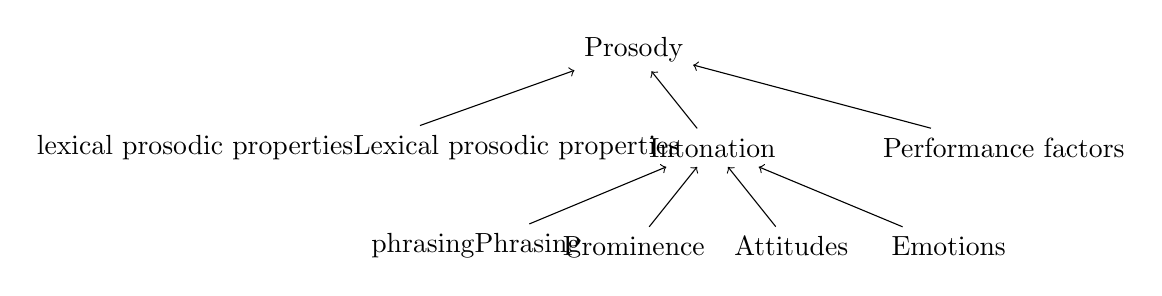
\begin{tikzpicture}
%	\node (a) at (0, 1) {\textsc{gen/num (erg)}};
	\node (b) at (1.5, 1.5) {\is{phrasing}Phrasing};
%	\node (c) at (1.5, 2.5) {\textsc{gen/num (erg)}};
%	\node (d) at (0, 2.75) {Lexically distinctive properties};
	\node (d) at (0, 2.75) {\is{lexical prosodic properties}Lexical prosodic properties};
	\node (e) at (3.5, 1.5) {Prominence};
%	\node (f) at (3, 1) {\textsc{gen/num (erg)}};
	\node (g) at (4.5, 2.75) {Intonation};
	\node (g2) at (8.2, 2.75) {Performance factors};
	\node (h) at (5.5, 1.5) {Attitudes};
	\node (i) at (7.5, 1.5) {Emotions};
%	\node (j) at (6, 1) {\textsc{gen/num (acc)}};
%	\node (k) at (9, 1) {\textsc{person (acc)}};
%	\node (l) at (9, -0.5) {Past \textit{\textbf{(Past Imperfect)}}};
%	\node (m) at (9, -1) {\textsc{person (acc)}};
	\node (n) at (3.5, 4) {Prosody};
	\foreach \from/\to in {g/h, g/i, n/d, n/g, g/b, g/e, n/g2}
	\draw [<-] (\from) -- (\to);
	\end{tikzpicture}
	\caption{A schematic representation of the components of {prosody}.}
		\label{fig:intonation}
\end{figure}

It should be emphasized that the tree-like diagram in \figref{fig:intonation} is a~highly simplified representation. It does not attempt to capture the subtle interconnections among the various components of \isi{prosody}, e.g.\ between \isi{rhythm} and lexically distinctive suprasegmentals. Its purpose is simply to provide a~visual summary of the core distinctions made here. The representation in \figref{fig:intonation} highlights the fact that \is{intonation|textbf}intonation is a~complex, abstract structure. Its four components can be grouped into two sets: 

\begin{itemize}
    \item Two sub-systems of linguistic structure: \isi{syntactic intonation} \textit{(\isi{phrasing})}, which primarily reflects syntax in the broad sense, and pragmatic intonation \textit{(\isi{prominence})}, which encodes \isi{information structure}; 
    \item Attitudinal and emotional dimensions, which convey speaker attitudes and emotions.
\end{itemize}

Speech \isi{phrasing} and \isi{pragmatics} are so central to intonation that it may be tempting to  define intonation exclusively in terms of these functions. As Rossi puts it: 
\begin{quotation}
    Thus, the role of a grammar of intonation would be to determine the structure of intonational categories and units linked in one way or another to syntax and semantics-pragmatics, in other words to identify the intonational forms governed by higher cognitive devices. \citep[105]{rossi_lintonation_2001}
        
    \medskip 
    %\footnote{
    {\noindent}\textit{Original text:} Ainsi une grammaire de l’intonation aurait pour rôle de déterminer la structure des catégories et des unités intonatives liées d’une façon ou d’une autre à la syntaxe et à la sémantique-pragmatique, en d’autres termes d’identifier les formes intonatives gouvernées par les dispositifs cognitifs supérieurs.
\end{quotation}
Indeed, one might argue that removing the expression of attitudes and emotions from \figref{fig:intonation} would not fundamentally alter the conceptual framework used here. Yet these last two components are essential to a~comprehensive understanding of intonation. Intonation, as Bolinger famously described it, is a~“half-tamed savage”
\citep[475]{bolinger1978}. \textit{Phrasing} belongs to the tamer, more intellectual, more structured domain; it is most clearly manifested in deliberate oral renderings of carefully composed texts. \is{prominence}\textit{Prominence}, though still describable within a~linguistic system and exhibiting clear cross-linguistic differences, is
a~less domesticated dimension of intonation: its stronger manifestations can at times interfere with \isi{phrasing} as dictated by syntactic structure. Finally, the expression of attitudes
and emotions transcends linguistic structure to some extent and can partly be accounted for in \is{ethology}ethological terms, for instance through the \is{Frequency Code|textbf}Frequency Code:
 
\begin{quotation}
{\dots}~an innately specified ‘Frequency
Code’ ({\dots}) associates high acoustic frequency with the primary meaning of ‘small vocalizer’ and thus secondary meanings as ‘subordinate, submissive, non threatening, desirous of the receiver's goodwill, etc.’ and associates with low acoustic frequency the primary meaning of ‘large vocalizer’ and such secondary meanings as ‘dominant, aggressive, threatening’, etc.\ \citep[1]{ohala1984}
\end{quotation}
	
Still on issues of terminological clarification, the phrase \is{syntactic intonation|textbf}“syntactic intonation” may appear to be somewhat of a~misnomer, insofar as intonational \isi{phrasing} does not stand in a~strict, one-to-one relationship with syntactic units. This has been recognized since the early classics of phonetics \citep{grammont1933} and has been further confirmed by later research
(\citealt{selkirk1972}; \citeyear[231]{selkirk2000}; \citealt{martin1981}). Nonetheless, the phrase “syntactic
intonation” is retained here, given that knowledge of a~sentence’s syntax provides
a~sufficient basis for the synthesis of an acceptable fundamental frequency {contour}
\citep{vaissiere1971}.

Rossi is led to consider that ``the primitives of intonation are two-sided signs: intonational morphemes" \citep{rossi_lintonation_2001}. This notion of \textit{intoneme} is reminiscent of Delattre's reflections, which distinguish between form and function: it is necessary to analyze ``on the one hand the significant oppositions that rely on intonation, and on the other the shape of the intonation curves" \citep[1]{delattre1966a}.\footnote{\textit{Original text:} «~{\dots}~d’une part les oppositions significatives qui reposent sur l’intonation, de l’autre la forme des courbes d’intonation~». The phrase ‘intonation curves’ might suggest that Delattre confines the phonetic dimension of intonation to fundamental frequency, which can be visualized as a curve. However, a~close reading his article~-- which is highly recommended~-- makes it clear that this is not the case.}
In terms of form, the acoustic correlates of \isi{prosody} are manifold. They include variations in fundamental frequency,
\isi{duration}, and intensity, as well as \is{phonation types}phonation type, but also allophonic variation in the realization of phonemes. Thus, \isi{prosody} has correlates at the respiratory (i.e.\ subglottal) level, the glottal level, and the supraglottal level (see \citealt{erickson1998}). All these parameters contribute to \isi{prosody} simultaneously, to varying degrees.

\subsection{Tone sandhi, morphotonology, and tonal morphology}
\label{sec:tonesandhietc}
\largerpage

The concepts of ‘{tone sandhi}’, ‘morphotonology’, and ‘tonal morphology’ also require clarification. \is{tone sandhi|textbf}\textit{Tone sandhi} refers to phonologically specified tone changes that apply automatically within a~given phonological domain. In other words, \textit{tone sandhi} refers to categorical tone change conditioned by phonological context. The seven tonal rules of Yongning Na presented in \sectref{sec:alistoftonerules} (reproduced below) are {tone sandhi} rules in this sense, as they govern adjustments among neighbouring syllables within a~given phonological domain (the \isi{tone group}).

	\begin{enumerate}[leftmargin=2cm, itemsep=0pt, labelwidth=\widthof{Rule~1:}]%[topsep=12pt, partopsep=0pt]
		\item[Rule~1:] L tone spreads progressively (“left-to-right”) onto syllables unspecified for tone.
		\item[Rule~2:] Syllables that remain unspecified for tone after the application of Rule~1 receive M tone.
		\item[Rule~3:] In tone-group-initial position, H and M are neutralized to M.
		\item[Rule~4:] The syllable following an H-tone syllable receives L tone.
		\item[Rule~5:] All syllables following an H.L or M.L sequence receive L tone.
		\item[Rule~6:] In tone-group-final position, H and M are neutralized to H if they follow an L tone.
		\item[Rule~7:] If a~\isi{tone group} only contains L tones, a~postlexical H tone is added to its last syllable.
	\end{enumerate}

\is{morphotonology|textbf}\textit{Morphotonology} refers to categorical change in tone governed by rules that are specific to particular syntactic phrase types, such as object plus verb, subject plus verb, numeral plus classifier, and so on. 

Finally, \is{tonal morphology|textbf}\textit{tonal morphology} refers to grammatically specified tone changes marking certain morphosyntactic categories. The phrase “tone cases” is used in descriptions of some \ili{Bantu} languages, such as \ili{UMbundu} \citep{schadeberg1986tone}, where a~noun's tone varies according to its case. 
%No less than twenty-five African languages that have tone cases are listed (and plotted on a~map) by \citet[225]{konig2008case}. 
The addition of a~specific tone to a~verb can express a~given tense-aspect-modality category. 
%Tonal morphology can further be divided into \textit{concatenative} and \textit{derivational} types. Concatenative tonal morphology consists in the addition of “tonal morphemes” (on the case of Saramaccan: \citealt{good2002, good2004}). 

In Yongning Na, there is no 
{tonal morphology} % Do not index, as the main (defining) index entry, with |textbf, sits on the same page.
in the sense of tonal morphemes. The \is{floating tone}floating High tone of Yongning Na is not a~morpheme (i.e.\ a~form-meaning pairing): it constitutes one of the lexical tone categories of nouns. Consequently, only the first two of the three concepts outlined above~-- 
%\is{tone sandhi}
sandhi, morphotonology, and tonal morphology~-- are relevant to the present study. 

Some authors adopt “a broad and loose usage of the term” \textit{sandhi}, encompassing both 
%\is{tone sandhi}
sandhi and morphotonology as defined here \citep[x]{chen2000}. While such an approach may be suitable for large-scale language surveys \citep[such as the survey of Chinese dialects in][]{chen2000}, distinguishing between sandhi and morphotonology is crucial in the present study. The reason for undertaking a~book-length description is that tonal alternations in Yongning Na are not purely phonological: alongside sandhi (as defined here, as a~phonological phenomenon), the language exhibits a~wide range of syntactically restricted \is{tone rules}tone rules~-- i.e.\ morphotonology. 


%\section[Intonation in level-tone languages: a look at \citet{guthrie1940}]{Intonation in level-tone languages: A~look at \citet{guthrie1940}'s study of Lingala}

% \section{Intonation in level-tone languages: A~look at African studies}
% \label{sec:literaturereviewintonationintonallanguages} xyz

%Before turning to intonation in Yongning Na, a~look at early research into intonation in level-tone languages appears useful to contextualize the discussion, continuing the above reflections about frameworks for studying intonation and crucial technical vocabulary. It also prepares the ground for the fledgling typological analyses set out in a later chapter (\sectref{sec:typologicalperspectives}).


%\subsection{Can intonation be described in terms of a~fixed number of levels?}


Based on these terminological clarifications, the next chapter (Chapter~\ref{chap:IntonationDescriptionAndAnalysis}) finally turns to intonation in Yongning Na. 



\is{intonation|)}
